%==============================================================================
% Section 1: Introduction
%==============================================================================
\section{Introduction}
\label{sec:intro}

\subsection{Background}
\label{sec:intro:background}

In papers~I--III/III (EC) \cite{paper1,paper2,paper3,paper3ec} we developed the
minisuperspace of Einstein--Cartan + Nieh--Yan theory through
topology-dependent phase classification, the homogeneous mode dictionary of
$\Sthree\times\Sone$, and the three-topology comparison among $\Tthree$,
$\Nilthree$, and $\Sthree$.  In paper~III (EC) \cite{paper3ec} the homogeneous
mode dictionary and the low-order EFT language were organised for both the
Levi--Civita and the Einstein--Cartan connections, providing a baseline for the
analysis of the homogeneous degrees of freedom.

These results, however, do not yet supply a single dictionary that surveys
``which response is allowed, protected, and activated in which geometry''
beyond the mode content of each individual geometry.  In particular, in order
to align inhomogeneous bulk responses, observables on boundaries/interfaces,
and cobordism-type comparisons between geometry pairs in a common convention,
one requires a comparison framework one level higher than the homogeneous
baseline.

The aim of the present paper is to construct this comparison framework
explicitly for the four Thurston \cite{Thurston1997} geometries $\Tthree$,
$\Nilthree$, $\Sthree$, and $\Solthree$.  The focus is not on re-deriving
individual modes but on presenting a response dictionary across the four
geometries together with selection rules that compress its content.

\subsection{Claims of the Present Paper}
\label{sec:intro:claims}

The central claims of this paper can be summarised in the following four
points.

\begin{enumerate}
  \item For the four Thurston geometries $\Tthree$, $\Nilthree$, $\Sthree$,
        and $\Solthree$, the Euclidean response can be systematised in two
        layers: a first-layer bulk and a second-layer boundary/cobordism.
  \item In the first layer a 36-entry bulk inventory closes together with
        geometry-dependent selection rules.
  \item In the second layer the three observable families
        spectral/torsional-charge/inflow close, and a pairwise cobordism
        dictionary is given for all six geometry pairs.
  \item The Euclidean circle admits two readings, the KK reduction reading and
        the Matsubara-style thermal reading, supplying the reduced description
        and the thermal description respectively.
\end{enumerate}

We contrast in particular the strict local APS spectral entry of $\Nilthree$,
the frame-bundle-normalised torsional-charge entry of $\Sthree$, the trivial
spectral benchmark of $\Tthree$, and the spin-sensitive global spectral branch
that arises on a compact $\Solthree$ benchmark.  Although $\Solthree$ is inert
in the CS direction count, it carries an EC slice minimum and a rigid
scaffold; in the boundary layer it forms a distinct entry that admits a
spectral branch depending on the compact quotient and the spin structure.

\subsection{Comparison Viewpoint}
\label{sec:intro:viewpoint}

The objects under comparison are the geometric responses defined on the
Euclidean product structure $M^3\times\Sone$.  Concretely, we treat the
homogeneous baseline of the four geometries, the inhomogeneous/nonlocal bulk
response, the boundary/cobordism observables, the pairwise cobordism
dictionary, and the two readings of the Euclidean circle.

The comparison admits three viewpoints.  The first is the geometry-wise
inventory obtained by examining each geometry in isolation.  The second is the
taxonomy that splits the observables into the three families
spectral/torsional-charge/inflow.  The third is the pairwise cobordism
dictionary based on the six pairs constructed from the four geometries.
Supplementing this with the geometric scaffold information allows one to
distinguish the class of an observable from the distinctness of the
background geometry.

\subsection{Outline}
\label{sec:intro:outline}

The paper is organised as follows.
Section~\ref{sec:baseline} fixes the homogeneous baseline that supplies the
common comparison axis for the four geometries.
Section~\ref{sec:bulk} gives the first-layer inventory of the
inhomogeneous/nonlocal bulk response.
Section~\ref{sec:boundary} organises the boundary/interface response into a
geometry-wise inventory, an observable taxonomy, a pairwise cobordism
dictionary, and a geometric scaffold layer.
Section~\ref{sec:rules} states the bulk--boundary selection rules as the main
result.
Section~\ref{sec:circle} describes the secondary readings of the Euclidean
circle, the KK reduction reading and the Matsubara-style thermal reading.
Section~\ref{sec:discussion} discusses the place of the present paper and its
future directions, and Section~\ref{sec:conclusion} concludes.  Appendices
collect notation conventions, complete inventories, KK--Matsubara coexistence
tables, the normalisation chain, and derivations.

\begin{figure}[H]
\centering
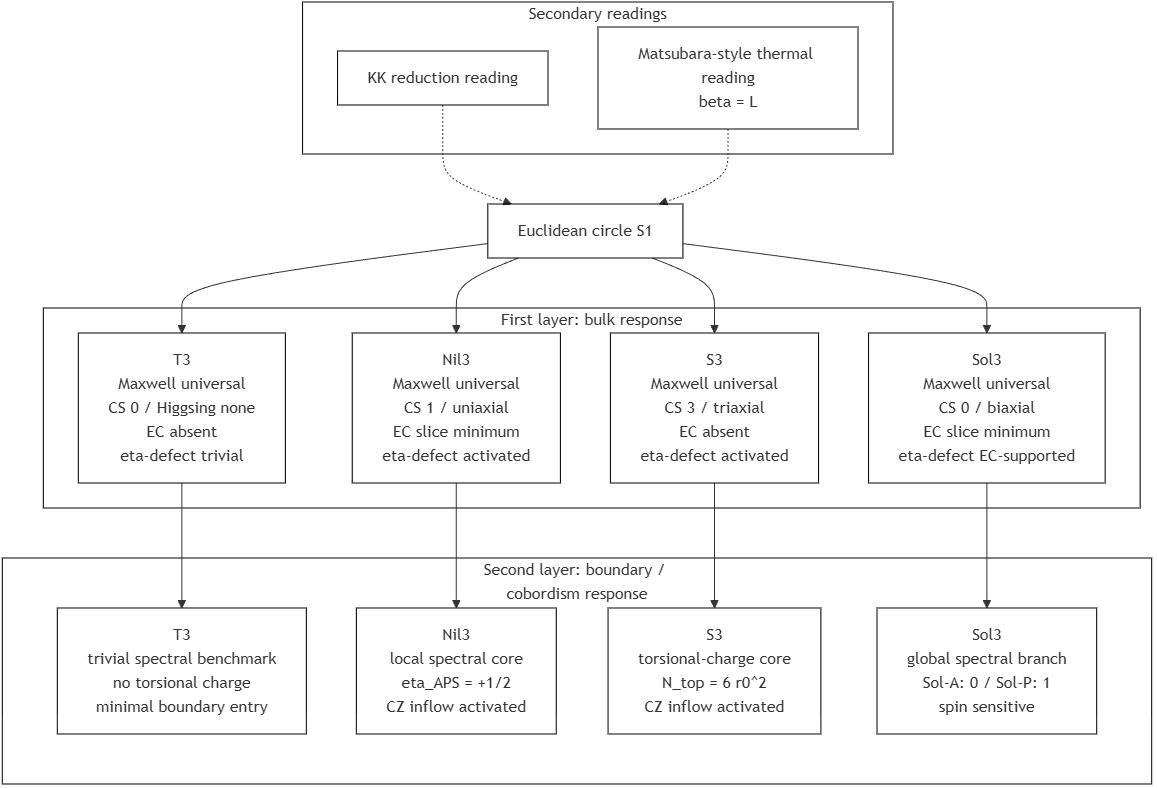
\includegraphics[width=0.95\linewidth]{figures/fig01_architecture_overview.png}
\caption{Two-layer architecture overview.  The first-layer bulk response and
the second-layer boundary/cobordism response are displayed along the four
geometries, while the KK reduction reading and the Matsubara-style thermal
reading---both arising from the same Euclidean circle---are separated as
secondary readings.}
\label{fig:architecture}
\end{figure}
